\documentclass[12pt]{article}
\usepackage{fullpage}
\usepackage{nopageno}
\usepackage{setspace}
\usepackage{acronym}
\usepackage{graphicx}

\author{Charles Pittman}
\title{AC Circuits}

\acrodef{AC}{Alternating Current}
\acrodef{DC}{Direct Current}
\acrodef{EE}{Electrical Engineering}
\acrodef{EMF}{electromotive force}

%\doublespacing
\onehalfspacing
\begin{document}
\maketitle

\section*{Introduction}

The study of electronics generally begins with exploring the function and
operation of \ac{DC} circuits, with skills learned then translated for \ac{AC}
circuits.  In that translation some students tend to focus more on applying the
formulas in problem solving, losing sight of how they were derived.  As a
result, they may have trouble describing exactly what \ac{AC} is and how it
works.

\section*{What is \ac{AC}?}

Recall that current flows only one way in \ac{DC} circuits.  Since the current
is moving in one direction the entire time the polarity of any terminal remains
constant.  As the name implies, current flows in alternating directions in
\ac{AC} circuits.  The current changes direction, so polarity between terminals
must change, thus voltage also alternates.

When plotted against time, an \ac{AC} current (or voltage) produces a
sinusoidal wave as shown in Figure~\ref{acwave} with one cycle (period) labeled
as $T$.  The period is used in defining another important value of the
waveform, frequency, determined to be the number of periods per second.

Note that the horizontal axis can be divided into angles using the fact that a
period in a sinusoidal wave is equal to $2\pi$ radians (or $360^\circ$).  As
the waves are periodic, when they fall out of phase, the difference occurs
through the whole wave.  This constant phase shift is labeled $\theta$ in
Figure~\ref{acwave}.  By relating this shift of phase to the angle divisions
along the axis, a phase angle is determined.

When referring to waveforms out of phase, it is common to determine one as
``leading'' or ``lagging''.  Like voltage, a leading or lagging waveform can
only be determined with reference to another value.  A waveform that starts its
cycle ahead of the reference is leading; likewise, one that starts later is
lagging.  By convention, voltage is used as the reference waveform in \ac{AC}
circuits.

\section*{How is \ac{AC} Generated?}

A simple model of a three-phase alternator is shown in Figure~\ref{alternator}.
It consists of a magnetic rotor, and spaced evenly around the stator are three
separate sets of coil windings.  As the rotor spins, an \ac{EMF} is produced,
in accordance with Faraday's Law, that changes polarity as each magnetic pole
passes over the windings.

Studying this motion, each value previously mentioned can be related, given a
single rotation is one full period.  If one revolution is a period, then the
number of revolutions in a certain amount of time must be the frequency.  Note
that since the windings are evenly spaced, there is an angle of $120^\circ$
between each, which is why each phase in a three-phase source is said to be
offset by $120^\circ$.

\section*{What is Complex Power?}

Impedance, the opposition of current in a circuit, is extended in \ac{AC}.  The
fields in capacitors and inductors continue to grow in \ac{DC} circuits until
large enough to stop current and voltage, respectively.  They function
similarly in \ac{AC} circuits, but discharge each time current changes
direction.

The sum of capacitance and inductance, referred to as reactance, describes the
energy stored in the circuit each cycle.  A purely reactive impedance causes
voltage and current to shift $90^\circ$ out of phase, causing the current to
return after only half a cycle.  Though there is no net flow through the
circuit, energy is still consumed because of the movement.

The power spent working against desired flow is termed reactive power and
plotted on the imaginary axis in Figure~\ref{complexpwr}.  The vector sum of
real power transferred and reactive power wasted, complex power, is what
actually reaches the load.

%\twocolumn
\begin{figure}[p]
	\centering
	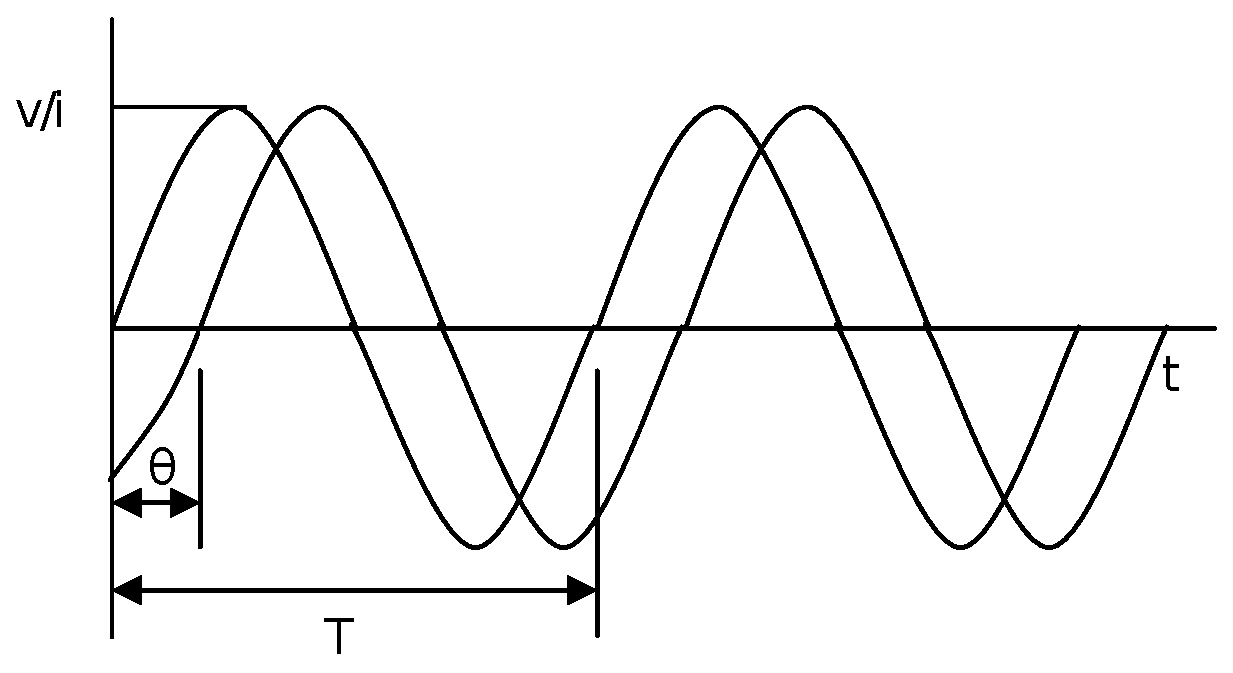
\includegraphics[width=0.6\textwidth]{img/acwave}
	\caption{Two Sinusoidal Waves With Phase Difference}
	\label{acwave}
\end{figure}

\begin{figure}[p]
	% ``Review of 3-Phase AC Circuits''  Not sure the university, but class
	% listed as EE340.  Author Y. Baghzouz.
	\centering
	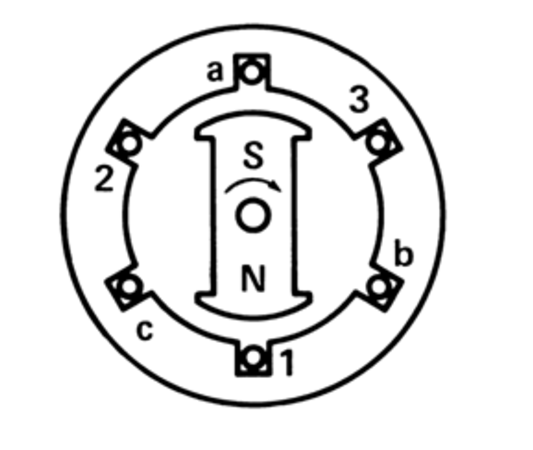
\includegraphics[width=0.4\textwidth]{img/threephasemotor}
	\caption{Simple Diagram of a Three-Phase Alternator}
	\label{alternator}
\end{figure}

\begin{figure}[p]
	\centering
	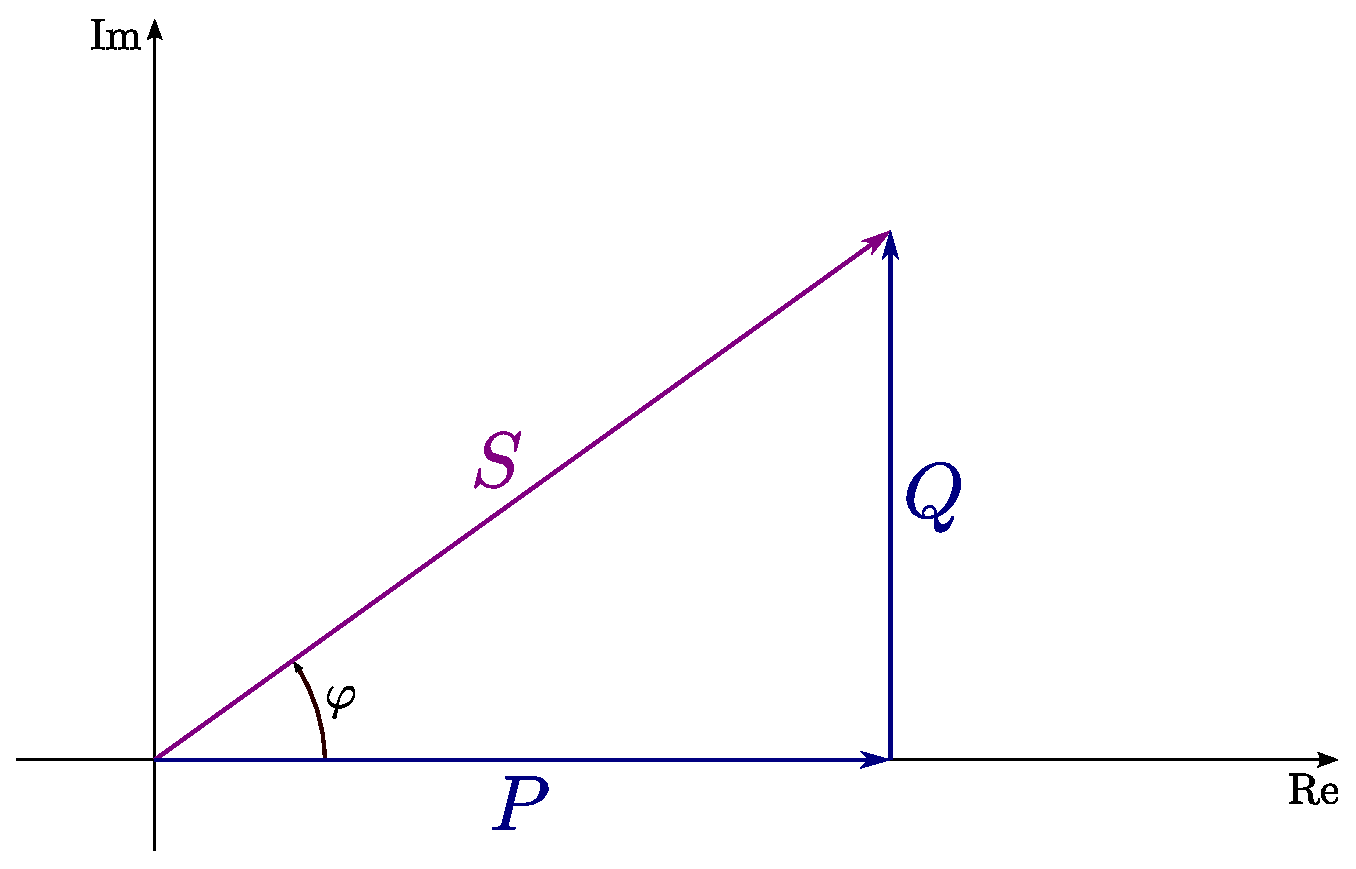
\includegraphics[width=0.5\textwidth]{img/complexpwr}
	\caption{Complex Power Triangle}
	\label{complexpwr}
\end{figure}

\end{document}
